Evaluados los distintos algoritmos, pasamos ahora a inspeccionar los mejores modelos encontrados para los clasificadores \textit{árboles de decisión}, \textit{linear discriminant analysis} y \textit{support vector machines}. En cada caso, vamos a buscar entender el comportamiento del algoritmo en función de aquellos hiperparámetros que regulan su complejidad; trazaremos curvas de aprendizaje, y sacaremos conclusiones en términos del sesgo y la varianza. Por último, dado que puede resultar de interés evaluar la aplicación de métodos de \textit{bagging}, vamos a realizar el mismo tipo de análisis para un modelo basado en \textit{random forests}.

El análisis se realizará de la siguiente forma: en base a las configuraciones obtenidas durante la etapa de búsqueda para cada clasificador, vamos a entrenar y evaluar una serie de nuevos modelos variando, por un lado, uno de sus hiperparámetros\footnote{En un rango relevante al mismo.} y, por el otro, la cantidad de datos\footnote{En el rango $[30, n]$ de a pasos de $10$.} de entrenamiento\footnote{Aclaramos que esta variación se realizó de manera acumulativa. Es decir, entre dos cantidades de datos consecutivas, sus correspondientes datasets $A$ y $B$ satisfacen $A \subset B$.}. La evaluación, igual que antes, se realizará por medio de $5$-fold cross-validation estratificado.

\subsection{Árboles de decisión}
Utilizando la configuración del modelo obtenido en la Figura \ref{random_tree}, generamos las curvas de complejidad ---sobre la \textit{altura máxima}--- y aprendizaje presentadas en la Figura \ref{decisionTreeComplexity}.  

Respecto de la complejidad, podemos apreciar que, a partir de una \textit{altura máxima} mayor a $7$, el modelo se acopla completamente a los datos de entrenamiento, indicando un sobreajuste. A su vez, sus respectivas performances en los datos de validación decrementan a partir de $\textit{altura máxima} = 4$ hasta estabilizarse en las alturas mayores a $8$. Esto podría indicar que el modelo ya separó todas las instancias en sus respectivas hojas, y dejó de cambiar sus reglas de corte. 
Podemos apreciar que durante la búsqueda aleatoria, la combinación con \textit{altura máxima} 4 no se probó, de otro modo se hubiese presentado como la mejor.

\vspace{0.5em}
\begin{figure}[!htbp] 
    \centering
    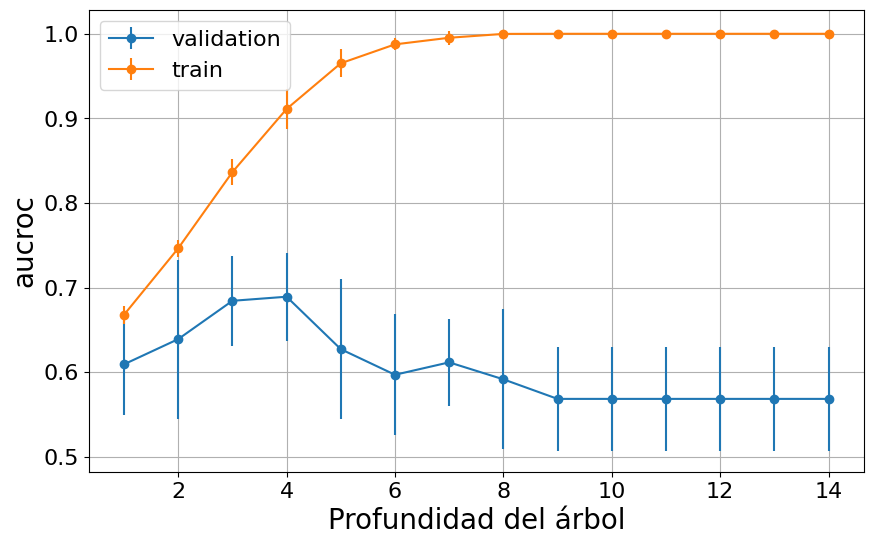
\includegraphics[width=0.4955\textwidth]{/files/src/.media/decisionTreeComplexity.png}
    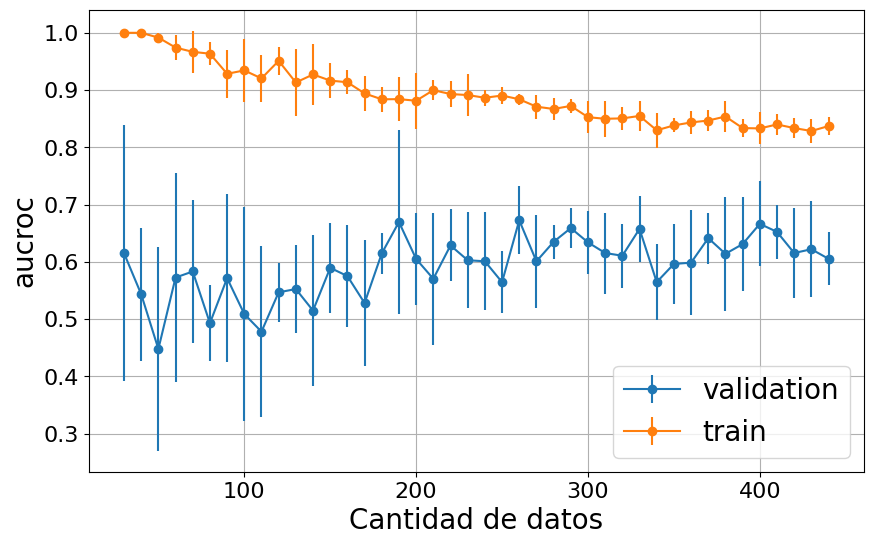
\includegraphics[width=0.4955\textwidth]{/files/src/.media/decisionTreeLearning.png}
    \caption{Clasificador \textit{decision tree}. Izquierda: Curvas de complejidad mostrando la variación del \textit{aucroc} a medida que se aumenta la \textit{profundidad máxima}. Derecha: Curvas de aprendizaje mostrando la variación del \textit{aucroc} a medida que se aumenta el tamaño del dataset.}
    \label{decisionTreeComplexity}
\end{figure}

Respecto a la varianza, podemos intuir que el rendimiento de este modelo va a cambiar considerablemente según el dataset utilizado en entrenamiento. Esto puede apreciarse en las barras de error\footnote{Estas corresponden a la desviación estándar de las mediciones de \textit{aucroc} para cada fold de validación.} presentes en la curva, donde en algunos casos, como para \textit{altura máxima} = 2 y 5, resultó en una diferencia de performance de más de un $10\%$ entre splits de validación. A su vez, puede verse cómo se van separando ambas curvas a medida que aumenta la \textit{profundidad máxima}. Es decir, la performance del modelo en entrenamiento aumenta mientras que en validación decrece. Esto muestra que la varianza del clasificador crece junto al hiperparámetro. El modelo parece acoplarse cada vez más al dataset.

Por otro lado, todos los resultados del algoritmo en validación se encuentran con un \textit{aucroc} por debajo de $0.75$, y con una media aproximadamente de $0.6$. En consecuencia, el modelo parecería tener poca capacidad predictiva. Sin importar el valor del hiperparámetro, es incapaz de acercarse a la distribución subyacente de los datos.

% 2. Graficar curvas de aprendizaje para cada modelo. En base a estas curvas, sacar conclusiones sobre si los algoritmos parecen haber alcanzado su límite, o bien si aumentar la cantidad de datos debería ayudar.

Por el lado de la curva de aprendizaje, podemos observar que, con pocos datos (menos de $150$ instancias), el modelo parece funcionar igual, a veces hasta peor, que un clasificador aleatorio, ya que su valor de \textit{aucroc} ronda el $0.5$ para validación. Al aumentar la cantidad de datos, ambas curvas se acercan entre sí, para luego estabilizarse en los valores de $0.85$ para el set de entrenamiento y $0.6$ para el de validación, lo que da cuenta de un sesgo moderado. Esto indicaría que el algoritmo, sin importar cuánto aumentemos el tamaño del set de entrenamiento, habría encontrado su límite de aprendizaje. 

\subsection{Linear discriminant analysis}
A partir de la configuración obtenida en la Figura \ref{lda}, generamos la curva de aprendizaje presentada en la Figura \ref{LDALearning}. En este caso, no vamos a considerar curvas de complejidad, ya que el algoritmo no cuenta con ningún hiperparámetro que, para nosotros, sirva como proxy para esta medida.

\vspace{0.5em}
\begin{figure}[!htbp]
    \centering
    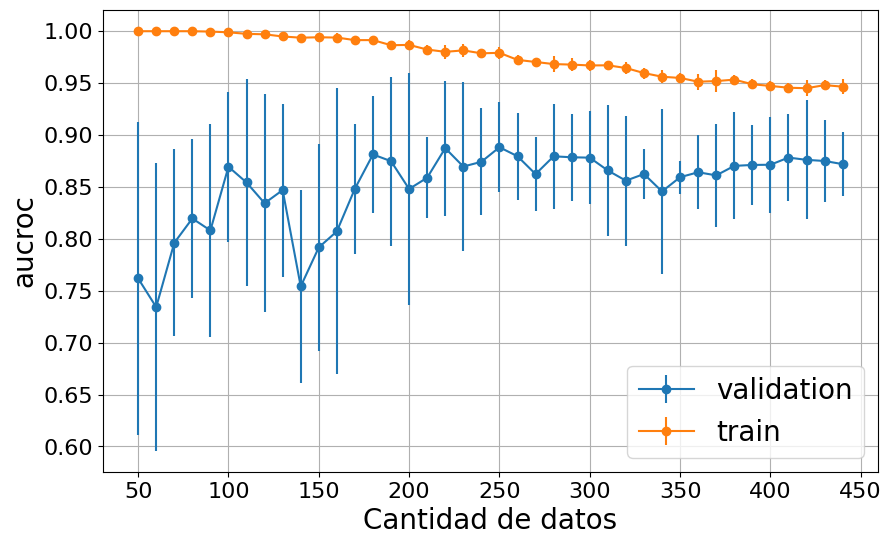
\includegraphics[width=0.49\textwidth]{/files/src/.media/LDALearning.png}
    \caption{Clasificador \textit{Linear Discriminant Analisis}. Curvas de aprendizaje mostrando la variación del \textit{aucroc} en datos de entrenamiento y validación a medida que se aumenta la cantidad de datos\protect\footnotemark.}
    \label{LDALearning}
\end{figure}
\footnotetext{Dado que durante la construcción de las curvas de aprendizaje se aumenta la cantidad de datos de entrenamiento, no nos pareció correcto resetear el \textit{random\_state} en el proceso de $5$-fold cross-validation estratificado que produce cada medición. Luego, los resultados pueden diferir un poco con respecto a los obtenidos durante la búsqueda aleatoria.}

Podemos apreciar que el modelo posee un sesgo bajo, teniendo en cuenta que su performance se estabiliza cerca del valor $0.87$ para validación, al contar con más de $200$ datos, y de $0.95$ para entrenamiento. Esto refleja que el modelo deja de aprender y, en consecuencia, contar con más datos no debería beneficiarlo significativamente. Como detalle interesante, notamos que el mejor valor de \textit{aucroc} luego de estabilizarse fue de $0.88$ para $250$ datos.

Por último, también se puede apreciar que al aumentar la cantidad de datos, la desviación estándar se achica, lo que parece indicar que la varianza del modelo diminuye. En general, el mismo parece poseer baja varianza desde los $200$ datos, en donde la curva se estabiliza. De manera tentativa, calculamos el promedio de las deviaciones estándar a partir de este tamaño de dataset, y su valor fue de aproximadamente $0.05$.


\subsection{Support vector machines}
Basándonos en la mejor configuración de hiperparámetros hallada (ver la Figura \ref{svm}), procedimos a realizar las curva de complejidad y aprendizaje presentadas en la Figura \ref{SVMCurves}.  La curva de complejidad utiliza el hiperparámetro $C$ como proxy. El mismo permite controlar la penalización por errores de clasificación. % Un valor mayor de C significa que el modelo penalizará más los errores de clasificación lo cual implica que buscará un hiperplano de separación que clasifique correctamente la mayor cantidad posible de ejemplos de entrenamiento. Por otro lado, un valor de C menor permite que el modelo tolere más errores de clasificación y puede resultar en un hiperplano de separación más general, incluso si esto significa clasificar incorrectamente algunos ejemplos de entrenamiento.

\begin{figure}[!htbp] 
    \centering
    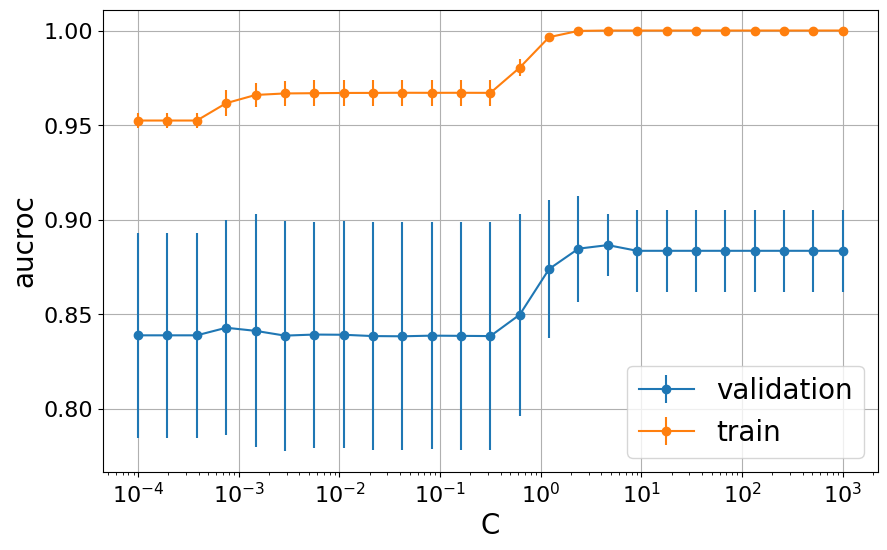
\includegraphics[width=0.49\textwidth]{/files/src/.media/SVMComplexity.png}
    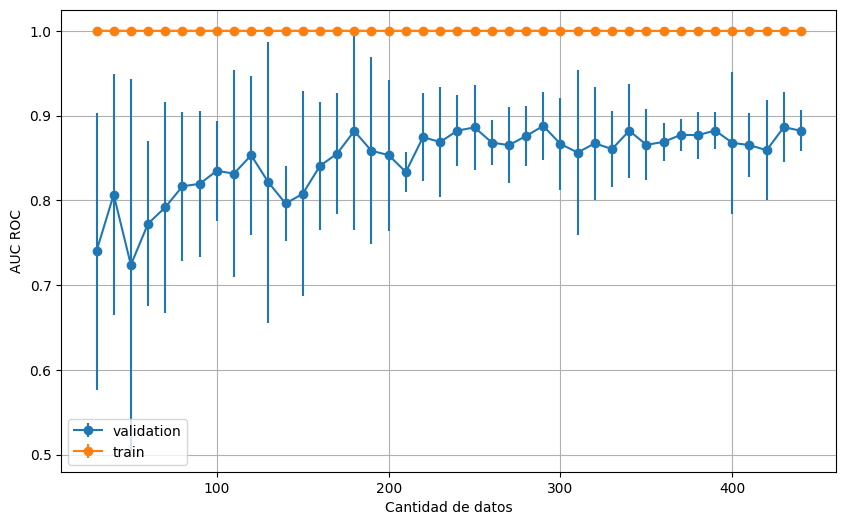
\includegraphics[width=0.49\textwidth]{/files/src/.media/SVMLearning.png}
    \caption{Clasificador \textit{SVM}. Izquierda: Curvas de complejidad mostrando la variación del \textit{aucroc} a medida que se aumenta \textit{C}. Derecha: Curvas de aprendizaje mostrando la variación de la medida respecto al tamaño del dataset.}
    \label{SVMCurves}
\end{figure}

Como se puede ver en la Figura \ref{SVMCurves}, el hiperparámetro $C$ afecta a la performance del algoritmo, aunque no de forma considerable. El mismo parece ser bastante bueno para modelar el problema, ya que sin importar el valor elegido para este parámetro, el \textit{aucroc} promedio es alto. De todas maneras, una elección incorrecta de $C$ parece causar una varianza alta dentro de los folds durante la validación cruzada, por lo que parece tener un mayor impacto en la estabilidad del modelo que en la performance.
 
Por su parte, la curva de aprendizaje en la Figura \ref{svm} nos permite determinar que la cantidad de datos es suficiente para armar un modelo decente, ya que a partir de los $250$ datos, pareciera mantener una performance constante. Algo a destacar es que, a diferencia de \textit{árboles de decisión}, la desviación estándar, incluso al considerar casi todos los datos, sigue mostrando una gran variabilidad, lo cual denota una posible inestabilidad del algoritmo. 

A partir de esta cantidad, se asienta un sesgo mediano, visible en la diferencia entre la curva de aprendizaje de entrenamiento y aquella de validación. El hecho que esta primer curva nunca baje de un valor de $1$ da indicios de una posible tendencia del modelo a sobreajustar. 

\subsection{Random forests}

Primero realizamos un Random Search para encontrar hiperparámetros decentes para Criterion y para maxdepth. Luego realizamos una curva de complejidad variando el maxfeatures, que nos serviría para entender como afecta este hiperparámetro a la performance del Algoritmo. 

\begin{figure}[!htbp]
    \centering
    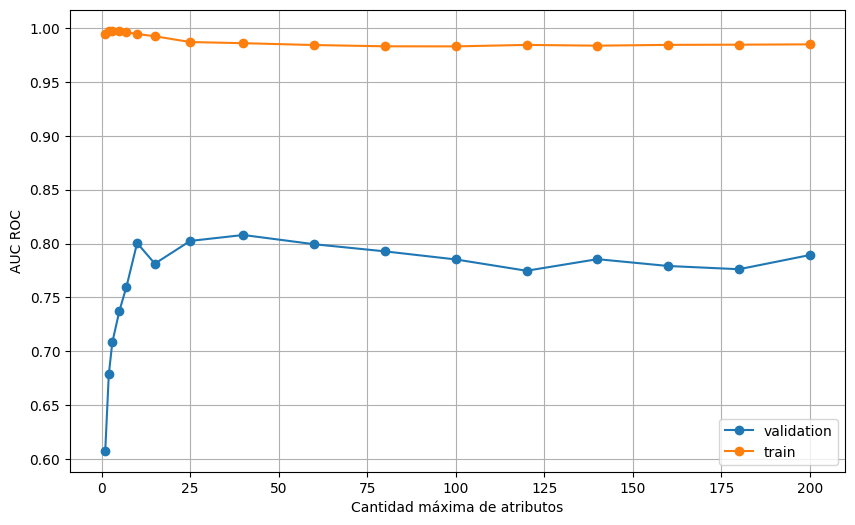
\includegraphics[width=0.49\textwidth]{/files/src/.media/randomForestComplejidad.png}
    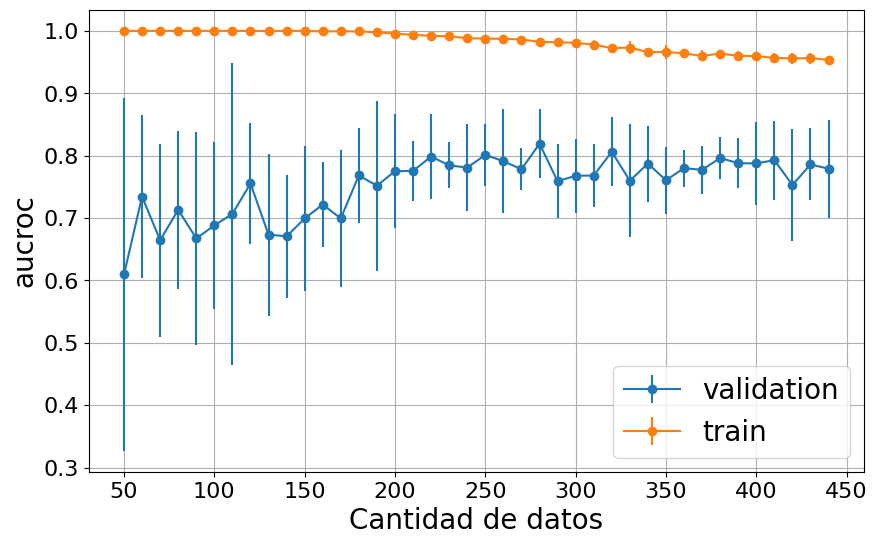
\includegraphics[width=0.49\textwidth]{/files/src/.media/randomForestAprendizaje.png}
    \caption{Clasificador \textit{Random Forest}. Izquierda: Curvas de complejidad mostrando la variación del \textit{aucroc} a medida que se aumenta \textit{maxFeatures}. Derecha: Curvas de aprendizaje mostrando la variación del \textit{aucroc} a medida que se aumenta el tamaño del dataset.}
    \label{RF}
\end{figure}

La figura \ref{RF} nos muestra algo que tiene sentido que es que cuando maxfeatures es muy bajo genera un impacto negativo en la performance del algoritmo. Esto tiene sentido ya que maxfeatures representa la cantidad de atributos tomados de manera aleatoria que cada decision tree que compone el forest va a considerar en cada paso del algoritmo. Es lógico que si considerás muy pocos atributos para realizar los cortes no encuentres buenas opciones y por lo tanto tengas un modelo defectuoso.

Por otro lado, la figura nos muestra otro resultado que no es tan intuitivo, que es que maxfeatures rápidamente alcanza su límite en el impacto en la performance y luego a medida que sigue aumentando, incluso pareciera decrecer ligeramente. Este resultado es particularmente atractivo, ya que si bien a medida que crece no mejora considerablemente la performance, si afecta directamente el costo computacional. 

La posible explicación para porque puede ser contraproducente tener un maxfeatures muy alto es que mientras más atributos se consideren en cada corte, menos variabilidad vamos a encontrar entre los árboles que componen el bosque. Es decir, los árboles resultantes van a ser más parecidos entre sí, lo cual genera un \textit{overfitting} de los datos.  

Concluimos que tiene sentido tomar logaritmo o sqrt de la cantidad de atributos de los datos para mantener maxfeatures dependiente de la cantidad de atributos, pero que sea realativamente bajo para tener una buena performance y minimizar la complejidad computacional.  

Por otro lado, graficamos una curva de aprendizaje (Figura \ref{RF}) para determinar si sería útil o no conseguir más datos. Lo que observamos a partir de la figura, es que a partir de 200 datos la performance del algoritmo parece mantenerse constante sin notar una tendencia alcista. Concluimos que la cantidad de datos provista es suficiente como para generar un modelo decente basado en random forest. 

Algo interesante a destacar de la curva de aprendizaje del random forest es que las barras de error son consistentemente pequeñas a medida que se aumentan los datos. 